\documentclass[a4paper]{article}

\usepackage[swedish]{babel}
\usepackage[utf8]{inputenc}
\usepackage{amsmath}
\usepackage{graphicx}
\usepackage[colorinlistoftodos]{todonotes}
\usepackage[margin = 0.8in]{geometry}
\usepackage{amssymb}
\usepackage{titling}
\usepackage{fancyhdr}
\usepackage{transparent}
\usepackage{eso-pic}
\usepackage{hyperref}


\newcommand{\mnamn}{Uppsala Datavetares GDPR-policy}

\AddToShipoutPicture{%
    \put(0,0){%
        \parbox[b][\paperheight]{\paperwidth}{%
            \vfill
            \centering {\transparent{0.05}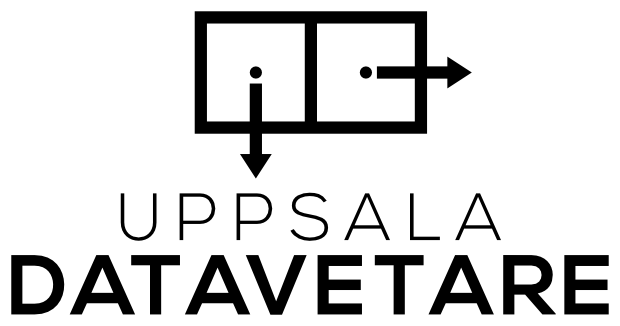
\includegraphics[width=1\textwidth]{UD_center.png}}
            \vfill
        }
    }
}


\title{\mnamn}


\date{}
\begin{document}
\maketitle

% \section{Integritetspolicy}
Antagen av Styrelsen 2021-01-28.

\abstract{
På sektionen Uppsala Datavetare (UD) värnar vi om din personliga integritet
och eftersträvar alltid en hög nivå av dataskydd. Denna integritetspolicy förklarar hur vi
samlar in och använder din personliga information. Den beskriver också dina rättigheter
och hur du kan göra dem gällande.
Det är viktigt att du tar del av och förstår integritetspolicyn och känner dig trygg i vår
behandling av dina personuppgifter. Du är alltid välkommen att kontakta oss vid
eventuella frågor.

Med hjälp av innehållsförteckningen nedan kan du lätt navigera till de avsnitt som är av
särskilt intresse för dig.}

\tableofcontents{}

\section{Policyns utsträckning}
Detta reglemente gäller Uppsala Datavetare (UD) inklusive alla organisationens utskott. Dessa hänvisas fortsättningsvis med beteckningen UD.

\newpage
\section{Vem är ansvarig för de personuppgifter vi samlar in?}
Sektionen Uppsala Datavetare, Lägerhyddsvägen 2 (Hus 1 2 TR), 75108, Uppsala är personuppgiftsansvarig för
organisationens behandling av personuppgifter.

\section{Varför behandlar vi dina personuppgifter?}
För att UD ska kunna bedriva sin verksamhet behandlas personuppgifter för olika
ändamål kopplade till verksamheten.
I det här avsnittet förklarar vi hur dina personuppgifter används för att vi ska kunna ge
dig relevant information om evenemang, tjänster och erbjudanden.

\subsection{Lagringstid}
  Om inget annat anges gäller följande:

  \begin{itemize}
    \item Vi sparar uppgifter om dig upp till 24 månader efter genomfört köp
    \item Vi sparar dina anslutningsuppgifter så länge du är ansluten till ett avtal
    \item Vi sparar dina personuppgifter i upp till 24 månader efter avslutat ärende/avtal för att säkra
      spårbarhet i din kommunikation med oss
    \item Vid lagring av medier sparar vi dina personuppgifter i upp till 25 år efter insamling av medierna, dessa arkiveras efteråt för historisk betydelse
  \end{itemize}



\subsection{När du köper biljetter till event eller handlar i våra kassor hanterar vi följande uppgifter som du lämnar till oss:}

\begin{itemize}
    \item Ditt namn (och namn på andra du agerar ombud för) och dina kontaktuppgifter
    \item Ditt personnummer, t ex när du köper eventbiljetter
    \item Din sektionstillhörighet om du uppger denna vid bokning/köp
    \item Uppgifter om behov av ledsagning eller rullstolsplats när sådana uppgifter
    behövs
    \item Uppgifter om betalning och betalningshistorik
\end{itemize}
\subsubsection{Vi hanterar dina personuppgifter för att:}
\begin{itemize}
    \item Identifiera dig som biljettinnehavare, t ex vid biljettkontroll
    \item Ta betalt för eventet, tilläggstjänsten eller varan, inklusive hantera
    kortbetalningar
    \item Hantera och leverera det du har köpt i enlighet med våra köpvillkor, t.ex. genom
    att tillhandahålla den produkt som du har köpt
    \item Meddela dig (via app, SMS, e-post eller liknande elektronisk kommunikation)
    om förändringar, t ex vid ändrade eventtider
    \item Marknadsföra våra event och produkter, t ex via e-post och sms
\end{itemize}



\subsubsection{Rättslig grund för hanteringen}
Vi hanterar dina personuppgifter med stöd i fullgörande av avtal när vi tillhandahåller
köpet och/eller produkten, med stöd av intresseavvägning när vi har ett berättigat
intresse att använda dina uppgifter för att marknadsföra våra tjänster,
säkerställa betalning och förhindra bedrägerier, samt med stöd i en rättslig skyldighet
för hantering av opt-out inställningar, ledsagning och rullstolsplats.




\subsection{När du är ansluten till avtal, prenumererar på mailutskick eller är engagerad:}
Uppgifter som du lämnar till oss såsom namn, personnummer och kontaktuppgifter, inklusive telefonnummer och e-postadress.



I avsnitten nedan kan du läsa mer om hur vi hanterar dina personuppgifter beroende på
om du deltar i ett event anordnat av UD, är ansluten till ett avtal och/eller prenumererar på mailutskick.

\subsubsection{Du som är ansluten till ett avtal}
När du är ansluten till ett avtal hanterar vi, utöver vad som beskrivs under
övriga punkter, även:
\begin{itemize}
    \item Uppgifter om din anslutning till ett avtal och din behörighet under avtalet
    \item Faktureringsinformation
    \item Uppgifter om din event och köphistorik
\end{itemize}

\noindent{}Personuppgifterna hanteras för att:
\begin{itemize}
    \item Administrera din anslutning till ett avtal
    \item Administrera betalning
    \item Säkerställa säkerheten för våra tjänster, för att upptäcka eller förhindra olika typer av olaglig användning eller användning som på annat sätt strider mot villkoren
\end{itemize}

\subsubsection{Rättslig grund för hanteringen}

Vi hanterar dina personuppgifter med stöd av intresseavvägning för vårt och den
avtalsanslutnas berättigade intressen att administrera och följa upp avtal.




\subsection{När du kommunicerar med oss}
Du kan välja att kommunicera med UD på många olika sätt, t.ex. via sociala medier, i
FAQ-forum, Tyck till funktioner eller i chatt, samtal och mail med någon representant
för vår organisation.

När du kommunicerar med oss hanterar vi uppgifter som du själv lämnar till oss t ex:
\begin{itemize}
    \item Namn och kontaktuppgifter
  \item Information om din synpunkt, fråga eller ärende
\end{itemize}

\noindent{}Vi hanterar dina personuppgifter för att
\begin{itemize}
    \item Besvara frågor och hantera ditt ärende, t ex avhjälpa fel, hantera klagomål och frågor om borttappade ägodelar
    \item Förbättra våra tjänster och den information som vi lämnar och publicerar via vår hemsida
\end{itemize}

\subsubsection{Rättslig grund för hanteringen}
Vi hanterar dina personuppgifter för vårt och ditt berättigade intresse att hantera ditt
ärende (intresseavvägning).


\subsection{När vi publicerar material på hemsida och sociala medier}

Vi publicerar i samband med de event som anordnas material på de sociala medier som
sammanknyter sektionen med dess medlemmar, samt på hemsidan och i nyhetsbrev i nyhetssyfte. Sektionens styrelse ska på begäran ta bort bilder på personer som inte önskar vara med på bild.


\subsubsection{Vi hanterar dina uppgifter för att}
\begin{itemize}
    \item Kunna dela bilderna till de som följer UD på sociala medier.
\end{itemize}

\subsubsection{Rättslig grund för hanteringen}

Vi hanterar dina personuppgifter med stöd av intresseavvägning när vi har ett
berättigat intresse att använda dina uppgifter för att kunna visa på att sektionen genomför
dess event och därigenom fullgör sitt syfte mot medlemmarna, samt ibland med
samtycke då detta insamlats på förhand och bilderna planerats användas vid
marknadsföringssyfte.

\subsubsection{Lagringstid}
Vi sparar dina personuppgifter i upp till 25 år efter insamling av bilderna, dessa arkiveras
efteråt för historisk betydelse.



\subsection{När vi har en skyldighet enligt gällande lagstiftning}

Utöver vad som beskrivs i punkterna ovan hanterar vi i vissa fall dina personuppgifter
när vi är skyldiga enligt lag, t ex på grund av vår bokföringsskyldighet, skyldigheter som
följer av trafikrättslig lagstiftning, eller vid begäran från myndighet.

\subsubsection{Rättslig grund:}
När vi hanterar dina personuppgifter på grund av att vi är skyldiga enligt lag gör vi det
med stöd i en rättslig skyldighet.

\subsection{Hur länge sparar vi dina personuppgifter?}

Dina personuppgifter lagras bara så länge som det krävs för att uppfylla ändamålen
med behandlingen, eller så länge som vi måste lagra dem enligt gällande lagstiftning.
UD kommer att genomföra en bedömning årsvis om ändamålet med behandlingen av
personuppgifterna kvarstår. Om inte ändamålen med behandlingen av
personuppgifterna kvarstår raderas eller avidentifieras dina uppgifter på ett säkert sätt,
så att de inte längre kan kopplas till dig.



\section{Företag som är självständigt personuppgiftsansvariga}

Vi delar även dina personuppgifter med vissa företag och föreningar som är självständigt
personuppgiftsansvariga. Att företaget/föreningen är självständigt personuppgiftsansvarig innebär att det inte är vi som styr hur informationen som lämnas till företaget/föreningen ska behandlas. Självständiga personuppgiftsansvariga som vi delar dina personuppgifter med är:

\begin{itemize}
    \item Statliga myndigheter (polisen, skatteverket eller andra myndigheter) om vi är
    skyldiga att göra det enligt gällande lagstiftning eller vid misstanke om brott.

    \item Företag som erbjuder betallösningar (kortinlösande företag, banker och andra
    betaltjänstleverantörer).
    \item Föreningar som anordnar evenemang som du deltar i tillsammans med UD
    \item Kårer och Nationer i Uppsala
    \item Uppsala teknolog- och naturvetarkår
\end{itemize}

När dina personuppgifter delas med ett företag eller förening som är självständigt
personuppgiftsansvarig gäller det företagets integritetspolicy och
personuppgiftshantering.



\section{Hur skyddar vi dina personuppgifter?}

Din integritet är viktig för oss och därför sätter vi säkerheten i fokus. Vi vidtar åtgärder
för att skydda dina uppgifter i enlighet med dataskyddsförordningen samt etablerade
riktlinjer för informationssäkerhet. Detta innebär att vi har rutiner och regler kring
dataskydd, t ex att vi skickar dina uppgifter på ett säkert sätt och säkrar att personalen
endast har tillgång till de uppgifter de behöver för att utföra sitt arbete.
I händelse av personuppgiftsincidenter har styrelsen skyldighet att inrapportera detta till
integritetsskyddsmyndigheten inom 72 timmar. Om det inte är osannolikt att medlem
riskerar att ta skada är kåren skyldig att informera de registrerade så de kan vidta
nödvändiga åtgärder.

Alla personuppgiftsincidenter ska dokumenteras.



\section{Dina rättigheter}
Rätt till tillgång
(s.k. registerutdrag) - Vi är alltid öppna och transparenta med hur vi behandlar dina
personuppgifter och ifall du vill få en djupare insikt i vilka personuppgifter vi behandlar
om just dig kan du begära att få tillgång till uppgifterna (informationen lämnas i form
av ett registerutdrag med angivande av ändamål, kategorier av personuppgifter,
kategorier av mottagare, lagringsperioder, information om varifrån informationen har
samlats in och förekomsten av automatiserat beslutsfattande).
Tänk på att ifall vi mottar en begäran om tillgång kan vi komma att fråga om ytterligare
uppgifter för att säkerställa en effektiv hantering av din begäran och att informationen
lämnas till rätt person.
Mer information om hur du kontaktar oss står längre ner i denna policy.

\subsection{Rätt till rättelse}
Du kan begära att dina personuppgifter rättas ifall uppgifterna är felaktiga. Inom
ramen för det angivna ändamålet har du också rätt att komplettera eventuellt
ofullständiga personuppgifter.

\subsection{Rätt till radering}
Du kan begära radering av personuppgifter vi behandlar om dig ifall:
\begin{itemize}
    \item Uppgifterna inte längre är nödvändiga för de ändamål för vilka de har samlats
    in eller behandlats.
    \item Du invänder mot en intresseavvägning vi har gjort baserat på berättigat intresse
    och ditt skäl för invändning väger tyngre än vårt berättigade intresse.
    \item Du invänder mot behandling för direktmarknadsföringsändamål.
    \item Personuppgifterna behandlas på ett olagligt sätt.
    \item Personuppgifterna måste raderas för att uppfylla en rättslig förpliktelse vi
    omfattas av.
    \item Personuppgifter har samlats in om ett barn (under 13 år) som du har
    föräldraansvaret för och insamlandet har skett i samband med erbjudande av
    informationssamhällets tjänster (t.ex. sociala medier).
\end{itemize}

Tänk på att vi kan ha rätt att neka din begäran ifall det finns juridiska skyldigheter som
hindrar oss från att omedelbart radera vissa personuppgifter. Dessa skyldigheter
kommer från bokförings- och skattelagstiftning, bank- och penningtvättslagstiftning,
men också från konsumenträttslagstiftning. Det kan också hända att behandlingen är
nödvändig för att vi ska kunna fastställa, göra gällande eller försvara rättsliga anspråk.
Skulle vi vara förhindrade att tillmötesgå en begäran om radering kommer vi istället att
blockera personuppgifterna från att kunna användas till andra syften än det syfte som
hindrar den begärda raderingen.

Mer information
Om du vill veta mer om dataskyddslagstiftningen och dina rättigheter kan du läsa mer
här:
\url{http://eur-lex.europa.eu/legal-content/SV/TXT/?uri=CELEX:32016R0679}
Om du skulle anse att vår behandling av dina personuppgifter inte sker i enlighet med
dataskyddslagstiftningen ber vi dig att kontakta oss, se avsnittet kontaktuppgifter
nedan. Du har även rätt att klaga till Datainspektionen som är tillsynsmyndighet.

\section{Kontaktuppgifter}

Uppsala Datavetare (org. nr. 8176065210) är
personuppgiftsansvarig för hanteringen av dina personuppgifter. Om du vill ha
ytterligare information om hur dina personuppgifter hanteras, kontakta oss genom
en skriftlig egenhändigt undertecknad begäran som skickas till: Uppsala Datavetare
Box 337, 75105 Uppsala. 
I brevet önskar vi att du uppger ditt namn, adress, e-post, telefonnummer samt
personnummer i tillägg till ditt ärende. Bifoga även en kopia av din legitimation. Svar
kommer att skickas till din folkbokföringsadress.

\section{Uppdateringar av informationstexten}

Denna informationstext uppdaterades senast den 24 januari 2021 och kan komma att
ändras. Om vi gör väsentliga ändringar i texten kommer vi meddela dig senast 30 dagar
innan ändringen träder i kraft genom e-post, sms, genom tjänsten, eller genom att
publicera en ny version på vår webbplats.



\end{document}

%%% Local Variables:
%%% mode: latex
%%% TeX-master: t
%%% End:
